\chapter{Literature Review} \label{cha:litrev}
In this chapter we will explore the theoretical background of our work, including research conducted on problems caused by current Android permission models, other solutions found and related work, and applications of trust transitivity in other domains.

\section{The Android Permission Model}
The Android permission model has been developed and updated since the introduction of Android as an operating system. In this section we will examine the theoretical applications of how the permission model is expected to provide privacy and security, and the methods used by similar systems to achieve better privacy protection.

\subsection{Comparison of Application Approval Process}

The leading mobile operating systems apart from Android are iOS by Apple, Windows Mobile and BlackBerry OS. Each of these have different processes and methodologies for developers to follow before submitting an application to the store. A comparison between application submission processes for these platforms shows that each has a centralized process for validation and/or verifying an application before it is made available for users to download. However these processes are usually in place for checking security or applications, and not privacy related issues. 
\smallskip

To submit an application to iTunes, the marketplace for iOS applications, the developer is first required to create an App ID and a Distribution Provisioning Profile and then  submit an application through iTunes connect with detailed information on the app.Three different certificates have to be submitted along with the application; the Distribution Certificate, Push Notification Certificate and Mobile Provisioning Certificate. The app has to be submitted through the Publication Center, where a checklist of complying standards that need to be adhered to has to be filled in.The approval process on average takes six days to one week.\cite{e}
\smallskip

Windows store applications also go through a centralized process before being released. A submission has to be created for each application with a checklist of information. Once the submission is complete and the application has been preprocessed without errors, it is submitted for certification through the Windows Certification Kit. The certification process focuses on three core areas; security tests, technical compliance tests and content compliance tests. The amount of time taken for an application to receive approval fluctuates based factors such as the code and logic complexity, visual content, rating of the developer, other applications in the queue etc. Applications which fail the certification process will be returned with a report indicating where the compliance standards were not met. Developers are allowed to resubmit applications following the same process.\cite{f}
\smallskip

RIM(Research In Motion) BlackBerry requires developers to submit applications for a complex process of reviewing, testing and "readying for publication" before being awarded a Approved/Up For Sale rating. Apps with this rating can be submitted and released on the BlackBerry marketplace; BlackBerry App World.\cite{j} 
\smallskip

Android developers add applications to marketplaces including Google PlayStore, Amazon AppStore, GetJar, SlideMe and F-Droid, which can then be downloaded by users. The problem lies in there being no centralized security measurement for applications on such marketplaces. Developers are trusted to prepare an application for release and then release it through a marketplace, email or website.\cite{g} The Android operating system imposes some security and privacy restrictions, including an install-time permission system, where each application declares what permissions it requires upon installation.\cite{h} This can provide users with control over their privacy since the choice to cancel installation lies with the user.

\subsection{Application Security and Privacy}
The Android OS is built on top of the Linux kernel, which manages the hardware including drivers and power management. From the bottom-up, the next layers include HAL or the Hardware Abstraction Layer, Native libraries and the runtime, which includes the Dalvik virtual machine, the framework with activity managers, system view and content providers, and a layer of applications(Refer Figure 2.1). Each time a new application is installed, the operating system assigns it a unique Linux user ID, which will be persistent for the lifetime of the application on that device. On uninstallation of an application, the user ID will be freed and possibly reassigned to another new application after the device is rebooted for the first time following an uninstallation.
\smallskip 

Permissions are tied to the user IDs, attemting to provide application sandboxing and process isolation by limiting communication between applications to methods overseen by the operating system such as passing of intents. Applications get a dedicated part of the file system connected to its UID whiich can be used to write private data and store databases and raw files, including permission information. According to the description on the Android Security website, the OS "seeks to be the most secure and usable operating system for mobile platforms by re-purposing traditional operating system security controls to protect user data, protext sstem resources and provide application isolation by providing robust security at the OS level through the Linux kernel, mandatory application sandbox for all applications, secure interprocess communication, application signing and application-defined and user-granted permissions"\cite{diagrameka}. However, this system has several loopholes, and malicious applications can access sensitive resources even in cases where sandboxing is done by the user ID system\cite{meshram2014survey}. 
\smallskip
\begin{figure}
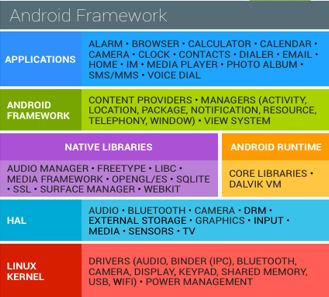
\includegraphics[totalheight=6cm]{Capture1}
\caption{The Android Software Stack}
\end{figure}
\smallskip

\subsection{Installing Applications}
The Android OS allows users to install both free and paid third party Java applications through markets such as Google Play. As discussed Android applications do not go through a review process to measure compliance to guidelines, although most competitors including iOS, Windows and RIM do. Access to sensitive resources, also known as "permissions" are controlled by the operating system to let aplications request access to sysytem functionality through an XML manifest, forming a computer-supported-access-system(CSAS)\cite{stevens2009computer}. Applications are allowed to define their own extra permissions in addition to the 134 core permissions provided by Android\cite{a}. (This research will not focus on third party defined permissions.)
\smallskip

Google Play application listings show information about each application including screenshots, marketing jargon, compatibility with user devices, app information, developer information, content rating, reviews and other related applications. However this does not include a list of permissions used by the app, or any privacy or security related information on the application page. Once a user clicks on the install button, they are expected to approve or disapprove the permission list that appears when downloading on devices older than Android M, without any background information. Permissions and privacy information are not highlighted on both the mobile application of Google Play or the store website\cite{kelley2013privacy}. 

\subsection{Before Android Marshmallow}
Before Android sdk 23, the permission model was based on a "do-or-die" concept. Users were given a list of permissions that would be required upon clicking the "install" link on an application on Google Play. There were no options to grant permissions selectively or revoke when not needed, and choosing not to grant a particular permission resulted in the application installation process being terminated\cite{felt2011effectiveness}. User choice was limited to whether they wanted to use the application, or not, and this has caused habituation even in later versions where permissions can be toggled\cite{wijesekera2015android}, since users choose to approve permissions by reflex as part of the installation process of an application. Research has shown that 83\% of application installations happen without the user consciously reading the permission list\cite{felt2012android}. Android Marshmallow is only being run on 10.1\% of all Android devices according the most current dashboard data at the time of writing\cite{androdashboard}, resulting in many users still being forced to follow the do-or-die model when installing applications(refer figure 2.2). 
%, width=0.5\textwidth
\smallskip
\begin{figure}
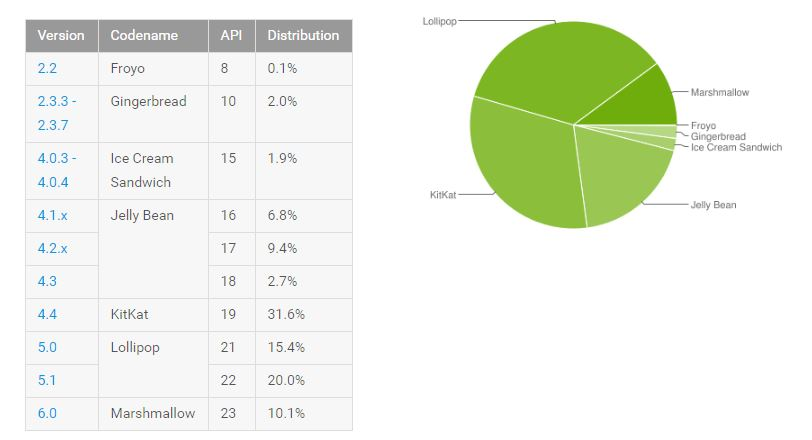
\includegraphics[totalheight=6cm]{Capture2}
\caption{Android Platform Versions as at 30.05.2016\cite{androdashboard}}
\end{figure}
\smallskip

\subsection{After Android Marshmallow}
The current permission model assigns permissions into two categories; normal permissions and dangerous permissions(See Appendix 01 for a list of normal and dangerous permissions). Normal permissions are granted automatically when requested by a user, and can alter basic low-risk elements of a device's settings, such as the display brightness or wallpaper. Dangerous permissions are any permissions that can alter sensitive data on the device or use the device's higher-risk functions, such as connecting to the Internet, and are further classified into groups. If a permission from the same group has previously been approved by the user, then the permission will be automatically granted(i.e. if READ\_SMS permission has been approved by the user then the device will not require permission to access the WRITE\_SMS permission either). However, if a dangerous permission is in a category which has not been approved by the user earlier, a popup notification is generated at runtime, asking the user to approve the permission request. The permission, once granted, can be revoked by toggling a control in the application settings page later on. However, it should be noted that there has been criticism of the classification of permissions, and may researchers such as Felt have pointed out in earlier experiments that the classification should be based on risk to user privacy\cite{felt2011android}, resulting in classification systems that do not correlate with what is currently implemented by Google\cite{androidyearinreview}. Refer figure 2.3 for a flowchart highlighting the recommended model for requesting permission in current Android devices.
\smallskip
\begin{figure}
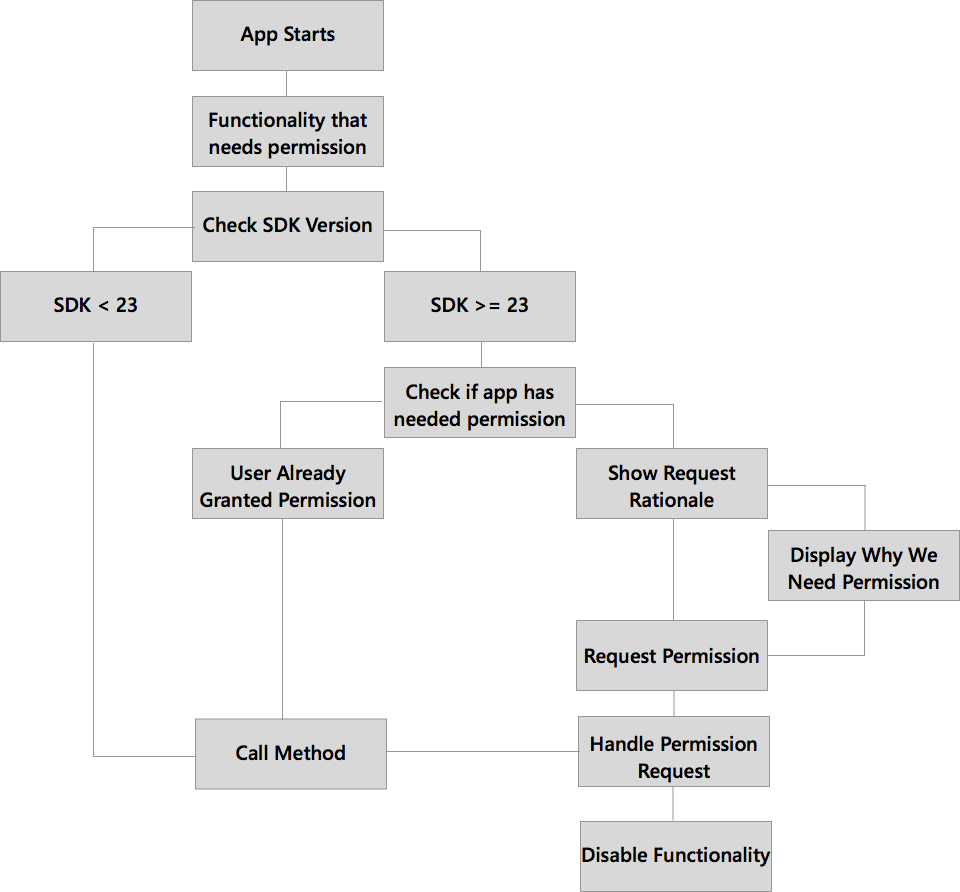
\includegraphics[totalheight=7cm]{Flowchart}
\caption{Android Permission Model- Flowchart\cite{flowchartimage}}
\end{figure}
\smallskip 

\section{Problems with the existing system}
The current permission model is problematic and offers loopholes that can be manipulated to compromise privacy of user data. This section will include a condensed view of research in this domain which highlight and offer solutions to some of these issues. 

\subsection{Least Privilege}
Both the most popular mobile operating systems, iOS and Android, require that developers follow the principle of "least privilege" with regard to permissions. The principle of least privilege states that "Every program and every user of the system should operate using the least set of privileges necessary to complete the job"\cite{schneider2004least}. In the context of Android applications, the principle states that developers should only ask for the very minimum of permissions that are required for the application to function\cite{enck2009understanding}. Applications on the Apple AppStore are screened to check adherence to this principle(and other factors) before being made available for download\cite{gilbert2011vision}. However since there is no such screening process for Android applications, research has shown that these permission guidelines are not generally adhered to by developers\cite{stevens2013asking}. Applications which do follow the permission guidelines are not necessarily popular with users, since permission requests either tend to be ignored due to lack of understanding\cite{felt2011android} \cite{kelley2012conundrum} or granted regardless of whether they are privacy sensitive or not due to habituation\cite{felt2012android}. This results in many popular applications not following the principle of least privilege\cite{wei2012permission}, with research showing that more than 33\% end up asking for more permissions than are required\cite{felt2011android}.

\subsection{Capability Leaks}
Applications can sometimes access permissions which are not requested at install time. Such violations of the permission architecture to access data are referred to as 'capability leaks' \cite{grace2012systematic} \cite{grace2011detecting}. A tool named Woodpecker, which analyzes each application to detect readability of permissions from unguarded interfaces, is frequently used in research in this domain \cite{zhou2012hey}. Through Woodpecker, two different types of capability leaks are identified; explicit leaks which find loopholes and access data without actually requesting permission and implicit leaks which let applications inherit permissions from another application, generally through intents. Other tools used to detect capability leaks include DroidChecker and IntentFuzzer \cite{yang2014intentfuzzer} \cite{chan2012droidchecker}. Capability leaks can also be exploited by malicious applications which use permissions which access permissions which have not been consiously granted to an application by a user for privilege escalation, using this to bypass restrictions on application functionality imposed due to the sand-boxing system\cite{davi2010privilege}.  

\subsection{Data Availability After Uninstallation}
Since application permissions once granted are not revoked even upon uninstallation of an application, the data collected through the permissions granted while the application was installed may still be accessible once the app is uninstalled. Upon uninstallation, the user identity belonging to the application is deleted, but the permissions allowed are not revoked, and data still exists as “orphans” without a unique identifier (or “parent”). These “orphans” may later be exploited by malware causing privacy breaches and leaking of sensitive data \cite{zhang2016life}. Users misunderstanding or choosing not to read permission requests before granting create lasting consequences, the effects of which continue to compromise privacy even after uninstallation of the problematic applications.

\subsection{Permission Creep}
Permission creep occurs in applications that do not follow the principle of least privilege and ask for extra permissions\cite{vidas2011curbing}. Applications may sometimes require permissions that are not required for the core functionality of the application, but rather due to revenue generation methods, since most 'free' applications available on the PlayStore require in-app purchases for extra functionality. Some of these 'free' and low cost applications may sell data to advertisers to generate revenue, without explicit permission from the user. Extra permissions may also be requested in cases where developers have difficulty trying to align permission requests with the functionality required for the application, resulting in genuinely having to request extra permissions that seems unnecessary on analysis, but are mandatory for certain functions \cite{vidas2011curbing}. For example an update for the popular game Angry Birds caused controversy by requesting permission to send SMS messages, which is not part of the expected functionality of the application. However Rovio (the company behind Angry Birds) later explained that this is due to the payment methodology needed to purchase new levels, where an SMS message is sent to Rovio from the device to be billed later by the carrier \cite{w} \cite{u}. 
\smallskip

Studies have shown that over 50\% of applications that request location access do so with the intent of sharing the information with advertisers for targeted marketing\cite{saint201050}. However, completely disallowing such requests would negatively impact the quality of applications available for Android since the revenue generation model would not survive. \cite{aa} In an ideal situation a user should be informed as to why an application is requesting a particular permission; as part of its core functionality, secondary functionality, as a method of revenue generation or any other usage for a permission to be requested. Research has shown that people tend to base their decisions on the reason behind data access\cite{lin2014modeling}. However this is not possible with the current model since the level of information made available to users regarding application permission requests is decided on by the developer.

\section{Proposed Solutions}
Apart from tools developed to identify and provide solutions to the issues discussed above, there have been several research related to alternate models or methodologies that could be followed to mitigate privacy risks in the current model.

\subsection{Facilitating Informed Decisions}
Barerra et al. have suggested hierarchical solutions, recommending a methodology for emperical analysis of permission based security models using Self-Organizing Maps(SOMs), with the intention of identifying potential points of improvement for the current model while increasing information flow conveyed through the permission dialog without creating additional complexity\cite{barrera2010methodology}. Models to breakdown functionality needed by Android applications to create a more fine-grained permission toggle than is available currently has been developed, allowing users to have more control over what data is accessed by an application, and when it is used\cite{bugiel2013flexible}. 
\smallskip

The current model does not allow users access to additional information as to why a particular permission is required, and studies have shown that this could be improved by analyzing human factors more effectively when allowing users to make such decisions. Research which focused on letting users choose applications based on their security and privacy expectations through including a "privacy facts" screen when downloading applications in addition to the list of permissions has proven that decisions made are different when users are given useful privacy information in addition to the current information provided\cite{kelley2013privacy}. Presenting users with personalized examples with their own data has also shown an increase in conscious decision making, and less habituation, for example by showing a sample of the users photos on the device and displaying "if you install this app, it will be able to access and delete the following of your photos" rather than just displaying the CAMERA permission\cite{harbach2014using}. 
\smallskip

Research has been carried out to design methods to recommend applications based on user's history of security and privacy concerns. Systems have been designed to track or reduce privacy violations by recommending applications based on users' security concerns\cite{almohri2014droidbarrier}. Tools have also been developed to track information flow on a device to determine "tainted" information and predict privacy violations in real time\cite{enck2014taintdroid}. Tools such as AppFence which give users the ability to track privacy violations and substitute fake data instead of actual user data for applications which violate privacy conditions have been developed, however this was not successful with all versions of Android and on average only worked for less than 33\% of privacy violations without crashing\cite{hornyack2011these}.

\subsection{Code Analysis to Curb Permission Creep}
Applications requesting unecessary permissions and causing permission creep can be analyzed through static code analysis, by using tools such as pScout\cite{au2012pscout}, and FlowDroid\cite{arzt2014flowdroid}. Static code analysis generally involves reading the Android Manifest and matching permissions which have been requested to those actually used by functions that provide core functionality of the application. Dynamic analysis of applications, runtime monitoring and Java code analysis have also been successful in identifying applications with permission creep \cite{spreitzenbarth2013mobile}. Context of a permission request; time of the request, whether the screen is on or off, whether the application is running visibly as a background or foreground application or service, what the device was displaying while the permission request was taking place, frequency of repitive permission requests(for example searching for network or wifi information) have been shown to influence users when deciding whether a particular permission request is appropriate \cite{wijesekera2015android}. This conforms to Nissenbaum's Theory of Contextual Integrity\cite{nissenbaum2004privacy} with regard to privacy, since the context and flow contribute towards the attitude of a user towards a privacy sensitive request, and not just information such as usage, reason etc.

\section{Transitivity of Trust}
